\section{Design}
\label{sec:design}

The design of the \lang{} compiler consists of two separate designs. The language
design and the compiler design. The language design is focused on the grammatical
structure of \lang{} where the compiler design focuses on the compiler and the design
of a software system capable of parsing the language as specified in the language
design.

\subsection{Language Design}
\label{sec:LanguageDesign}

\lang{} is an expression based language. This means that nearly every language construct
evaluates to some value\cite{Expr-Lang}. This is the driving principle behind
\lang{} together with a principle of immutability which means that every variable in
\lang{} is immutable unless they are explicitly declared to be mutable. \\ 

\lang{} further enforces a few rules to ensure the
type safety and memory safety of \lang{}. First \lang{} is a strongly and statically
typed language, meaning all types must be knowable at compile time and cannot be
changed at runtime. Secondly, it enforces the same principles of borrowing and
references that the Rust programming language enforces, in so far that \lang{}
currently supports language constructs that require the enforcement of Rust's
rules\footnote{Example: \lang{} currently does not support heap allocations therefore
the principles of Rust's borrowing and reference system pertaining to such allocations
are not yet enforced by \lang{}}.

These principles all together ensures a solid foundation for a language that can
achieve the goals of this project; to design a language which encourages clarity in
its code, while also offering type safety and memory safety when dealing with
allocation of memory.

\subsubsection{Grammar}

The grammar of \lang{} is quite simple, and is heavy inspired by the grammar of the
Rust language, however its grammar is also influenced by its limited feature set. 

Due to time constraints \lang{} does not support multiple files, this constraint
influences the way \lang{} is designed. Unlike scripting languages like
\texttt{Python} and \texttt{JavaScript}, which are capable of running its code without
a dedicated main function \lang{} organizes its code similarly to procedural
languages like \texttt{C} in which a main function is required for a standalone
program. \\

Because \lang{} is entirely constrained to a single file its grammar is designed to
help and encourage users to modularize their code through the use of functions but it
also limits its scalability as it becomes impractical to write large application
using \lang{} as this would lead to an unmanagable large file. \lang{}'s structure
can be broken down into three levels of abstraction. The \texttt{Program} layer, the
\texttt{Function} layer, and the \texttt{Expression} layer. Each layer is defined as
simplification of the layer below it. This will be detailed in the following
sections, but for a complete overview of the \lang{} grammar and production rules see
appendix~\ref{sec:syntax}.

\paragraph{Program Layer}\hfill 
\vspace{.3em} \hfill

The \texttt{program} layer, defines the highest level of abstraction in \lang's grammar. 
It is considered an expression like all other language constructs and it's values is
the value of the last expression in the program\footnote{which will typically be the
return value of the program's main function.}. \\

\newpage

In BNF notation, the grammar associated with the \texttt{program} layer is defined as follows:

\lstset{
  escapeinside={(*}{*)},
}

\begin{lstlisting}[caption={Program Layer}, label={lst:ProgramLayer},
frame={single}]
  <program> ::= <function_list>

  <function_list> ::= (*$\epsilon$*)
                  |   <function_list> <function_decl> 
\end{lstlisting}

At the highest level this generally means a the program will take the following form: 

\begin{lstlisting}[caption={Program layout}, label={lst:ProgramLayout}, frame={single}]
  fn function1(): int { // implemenation left out for brevity }
  fn function2(): int { // implemenation left out for brevity }
  fn main(): int { // implemenation left out for brevity }
\end{lstlisting}

With the main function being the entry point of the program calling the other
functions which in turn may be calling each other. It is important to note that
\lang{} does not support the use of functions before they are declared, meaning that
the order of the functions in the program is important. Thus \texttt{function1}
cannot call \texttt{function2} in the example above, but \texttt{function2} can call
\texttt{function1}. \\

Like other languages, such as \texttt{C} and \texttt{Rust}, where the main function is required for a
standalone program, \lang{} also mandates a main function. However, in scenarios
where \lang{} is utilized as a library for \texttt{C} or \texttt{C++} code, the main function is not
necessary. In such cases, the entry point is provided by the host \texttt{C} or
\texttt{C++} application, leveraging \lang{}'s functionality without the need for its own main
function. This distinctive feature, facilitated by the integration with the \gcc{},
allows for greater versatility in how \lang{} can be applied. More
details on this integration are provided in Section~\ref{sec:CompilerDesign}.

\paragraph{Function Layer}\hfill 
\vspace{.3em} \hfill

The \texttt{function} layer defines the second highest level of abstraction in 
\lang's grammar and togehter with the \texttt{expression} are abit more complicated
that the program layer. 
This layer defines how a function is declared and implemented. \\

On a high level, a function declaraction in \lang{} is a way to name what are called
block expressions, which are blocks of sequentially evaluated expressions that are
evaluated when the function is called. A function evaluates to the value of its
return expression(s)\footnote{A function can have multiple return expression in the
case of conditional return expressions.}. \\

In BNF notation, the grammar associated with the \texttt{function} layer is defined as follows:

\begin{lstlisting}[caption={Function Layer}, label={lst:FunctionLayer}, frame={single}]
  <function_decl> ::= 
    FUNCTION IDENTIFIER LPAREN <arg_list> RPAREN COLON TYPE <exprBlock>

  <arg_list> ::= (*$\epsilon$*)
                | <arg_list> ',' IDENTIFIER COLON TYPE
                | <arg_list> ',' IDENTIFIER COLON TYPE_REF
                | IDENTIFIER COLON TYPE
                | IDENTIFIER COLON TYPE_REF


  <exprBlock> ::= LBRACE <expr_list> RBRACE

  <expr_list> ::= (*$\epsilon$*)
                | <expr_list> <expr> END_OF_LINE
                | <expr_list> <if_expr>
\end{lstlisting}




\newpage

\subsection{Compiler Design}
\label{sec:CompilerDesign}

As both the \lexer{} and the \parser{} are generated by thirdparty tools these will
not be covered in any greater details but a full table of the tokens and the
production rules can be found in appendix~\ref{sec:appA} and \ref{sec:appB}. To best
understand the design of the \static, its components: the type checker and the borrow
checker as well as the \codeGen{} requires understanding of
the visitor pattern as well as the structure of the \ast{} of a typical \lang{}
program.

\subsubsection{Understanding the AST}
\label{sec:AST}

The \ast{} of a typical \lang{} program can typically be divided into three
sections; the program layer, the function layer and the expression layer (see
figure~\ref{fig:astStruct}). Each node in the \ast{} correspond one-to-one with a
type of expression in \lang{} but without loose of generality they will just be
refered to as nodes.

\begin{figure}[ht]
  \centering
  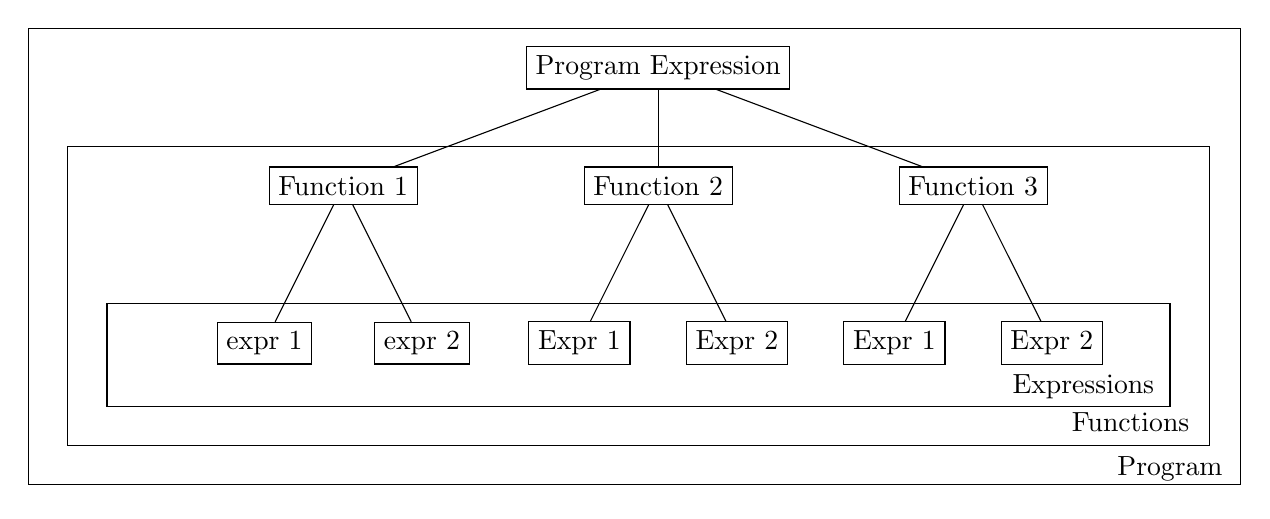
\begin{tikzpicture}
    \node[draw] (program) at (0, -0.5) {Program Expression};

    \def\functions{{Function 1}, {Function 2}, {Function 3}};
    \def\instructions{{Expr 1}, {Expr 2}}

    \foreach \fun [count=\i] in \functions {

      \pgfmathtruncatemacro{\x}{(-8 + (\i)*4)};
      \node[draw] (func\i) at (\x, -2) {\fun};
      \draw[] (program) -- (func\i); 

      
    }

    \node[draw] (int1) at (-5,-4) {expr 1};
    \node[draw] (int2) at (-3,-4) {expr 2};

    \draw[] (func1) -- (int1);
    \draw[] (func1) -- (int2);
    
    \node[draw] (int3) at (-1,-4) {Expr 1};
    \node[draw] (int4) at (1,-4) {Expr 2};

    \draw[] (func2) -- (int3);
    \draw[] (func2) -- (int4);
    
    \node[draw] (int5) at (3,-4) {Expr 1};
    \node[draw] (int6) at (5,-4) {Expr 2};

    \draw[] (func3) -- (int5);
    \draw[] (func3) -- (int6);
 
    \draw[] (-8,0) rectangle (7.4,-5.8);
    \draw[] (-7.5,-1.5) rectangle (7,-5.3);
    \draw[] (-7,-3.5) rectangle (6.5,-4.8);

    \node[] (programBox) at (6.5, -5.6) {Program};
    \node[] (functionBox) at (6, -5) {Functions};
    \node[] (instructionBox) at (5.4, -4.55) {Expressions};
  \end{tikzpicture}
  \caption{\ast{} for \lang{} showing how a typical program is structured after
  being parsed by the \lang{} parser. Each expression node, can then be further
subdivided until leaf becomes a terminal expression.}
  \label{fig:astStruct}
\end{figure}

It is this structure on which the \typeChecker, the \borrowChecker, and the
\codeGen{} will operate to produce and object file which the \gcc{} can turn in to
machine code. The use of the visitor pattern (see section~\ref{sec:VisitorDesign}) is
specifically used to facilitate a depth first left to right walk through of the \ast{} to do
type checking, borrow checking and gode generation.

This ensures the code is analyzed in the same order in which it appears in the
source code.

\subsubsection{Visitor Pattern}
\label{sec:VisitorDesign}

As can be seen on figure \ref{fig:CompilerProcess}, several steps in the compilation process acts on the \ast{}, with semantic analysis containing both a \typeChecker{} and a \borrowChecker{} evaluating the \ast{}, and the code generator running through the \ast{} to generate the intermediate representation.\\
As the Compiler has to traverse the tree several times, it would be desirable to have
a unified way of traversing the structure for all the different steps. The immediate
and naive solution would be to implement the different algorithms into the tree nodes
directly. This approach has the appeal of making it easy to add new nodes. It does,
however, make it difficult to add additional functionality to the compiler, as every
addition requires a modification of every node class. It also requires that the nodes
transmit information between each other, causing high coupling. A better solution
would be to use the visitor design pattern. \\

The visitor pattern separates algorithms from an object structure by implementing a 'visitor' class which can traverse the tree and perform the correct operations on each node. This allows for additional functionality to be added, without modifying the existing tree (thus following the open-closed principle). As long as every node implements an 'accept' function, new visitors can be added without the need for altering the expression classes at all. A modification of the \ast{} is necessarily more involved when using a visitor, compared to the naive approach, as every visitor must be updated to handle the new type of node, but the structure makes it easy to see where the changes should be made. 

\begin{figure}[h]
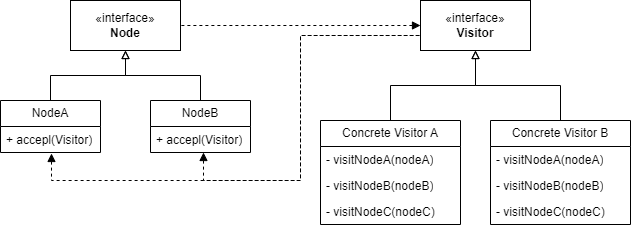
\includegraphics[width=\textwidth]{02-Body/Images/VisitorClassDiag.png}
\caption{Class diagram for Visitor Pattern}
\label{fig:VisitorClassDiagram}
\end{figure}

Figure \ref{fig:VisitorClassDiagram} shows a class diagram for a visitor design. The nodes of the tree all inherit an accept function from the Node interface, which takes a visitor interface as a parameter. The sole purpose of this accept funtcion is to call the correct visit function in the given visitor (nodeA calling visitNodeA(...) etc.). The Concrete visitors inherit Visit functions (visitNodeA(...), visitNodeB(...) etc.) from the Visitor interface, with each visit function taking the corresponding node type as a parameter. The actual functionality is the implemented in the visit functions, and because they have been given the actual node as a parameter, all relevant information is readily available.


\subsection{Type Checker}
The type checker implements a visitor, as described in section \ref{sec:typeCheckerDesign}. To the types available are \textit{int}, \textit{float}, \textit{char} and \textit{bool}. To keep track of the type of each expression, the base expression (that all expressions inherit from) was given an attribute "type", with public get and set functions. The types where denoted with string types. It was considered using an Enumerator, but in order to get usable error messages from the \lang{} compiler, it was necessary to have the types as string anyway. Having the types as strings also allows for easy expansion of the number of permitted types, as only terminal expressions determines type.\\
Variables are handled with a symbol table that maps the variable identifier to its type. As it is possible to have several variables with the same name if they are in different scopes, the symbol table is actually implemented as a stack of maps, each corresponding to  a single scope. This is explained in more detail in section \ref{sec:CodeGenImplement}, as it is the same technique used in Code Generation.\\
\subsubsection{Type in AST}
The code generator and borrow checker need to know the types of certain expressions, which poses a small problem. Most expressions do not know what their type is. I.e. a binary expression knows only which two expressions to work on, but not what type they are. Only terminal expressions know their own type. In order for the borrow checker and code generator to work, each expression therefore must be given a type. This task falls to the typechecker. As it checks that the type safty is kept, it calculates the type of every expression, and, once certain that the expression does not violate type safety, sets the type field in the expression to the calculated type.\\
This introduces a bit of coulpling, as the later modules depend on the typechecker setting the types in the AST, but the alternative is to calculate the types when creating the tree, and again in the typechecker, it was decided that a slight coulping was preferable to this double work. It is of coures still possible to use the modularity that the visitor pattern gives, as one can easily still swap the typechecker with another, as long as the new typechecker also writes the types to the AST.
 
\subsection{Borrow Checker}
\label{sec:BorrowCheckerImpl}

The \borrowChecker{} implements the visitor pattern, as described in
section~\ref{sec:VisitorDesign}, and uses two tables; a
\texttt{symbolTable} and a \texttt{referenceTable} to keep track of variables as well
as keeping track of references, as described in
Section~\ref{sec:BorrowCheckerDesign}. The \borrowChecker{} then uses these tables to enforce the
same ownership, borrowing and reference rules as the \texttt{Rust} language as described
in section~\ref{sec:LanguageDesign} and section~\ref{sec:BorrowCheckerDesign}. \\

\todo{re-write snippet to add more to the implementation instead of discussions}

Consider the code snippet as provided in listing~\ref{lst:referenceExample}. When the
\borrowChecker{} needs to evaluate if a reference assignment is legal, it retrieves
the a list of existing references to the variable that is being referenced from the
\texttt{referenceMap} and then does some checks to ensure that the \ast{} is in
compliance with the rules laid out in section~\ref{par:Ownership}.

\begin{lstlisting}[
  language=c++,
  numbers=left,
  frame=single,
  caption={Code showing a snippet of the referenceAssignment function in the \lang{}
  \borrowChecker{} implementation},
  label={lst:referenceExample},
  showstringspaces=false,
  ]
  ... // validation of the existence of the referenced variable 
  ... // cut out for brevity. 

   std::vector<std::pair<std::string, bool>> &vec =
      referenceMap[variable->getReferenceIdentifier()]; 

  int mutableCount = 0;
  bool hasImmutable = false;
  for (const auto &pair : vec) {
    if (pair.second) {
      mutableCount++;
    } else {
      hasImmutable = true;
    }
  }

  if (mutableCount > 1) {
    throw std::invalid_argument(
        "Invalid argument: more than one mutable reference");
  } else if (mutableCount == 1 && hasImmutable) {
    throw std::invalid_argument(
        "Invalid argument: mixed mutable and immutable references");
  }
  ...
\end{lstlisting}

This implementation is only responsible for tracking references inside a single
function scope, the implementation gets more difficult when tracking variables
between function scope and the current implementation of the \borrowChecker{} does
not yet accomplish this leading to correct programs throwing compile time errors when
they should. \\

The issue here seems to stem from an issue of correctly tracking and removing
variables from the \texttt{symbolTable} and the \texttt{referenceTable} when the
scopes are not nested inside each other.


\subsection{Code Generator}
\label{sec:CodeGenImplement}
This is where the visitor pattern truly comes into its own. Whereas the borrow and type checker each performs limited operations on each node, which could feasibly be performed by e.g. the nodes constructors, the code generator is sufficiently complicated that it requires its own structure to avoid loosing the overview. This is of course beside any consideration of coding principles.\\
When writing the code generator we have taken inspiration from the LLVM tutorial
language Kaleidoscope\cite{LLVMTutorial} to see how to set up boilerplate and as a
starting point when looking for the correct LLVM functions.

\subsubsection{LLVM}
LLVM works with three important components: a Builder, a Context, and a Module. The Builder provides an API to create the program instructions, the Context manages the core global data (types, code blocks and program instructions created by the builder), while the Module stores the functions.

\paragraph*{Variables}
When the Builder creates a program instruction, it usually returns an llvm::Value type. It is possible to store these in a \texttt{symbolTable} and access them later, but because LLVM creates a static single assignment IR, it is not possible to change the value of the stored variables. To get around this we create an allocation instance (llvm::AllocaInst), which can hold an llvm::Value. We can then store new llvm::Values in the same llvm::AllocaInst, obtaining mutable variables. The exact implementation is shown in listing \ref{lst:varAssignment}.

\begin{lstlisting}[
  language=c++,
  frame=single,
  numbers=left,
  caption={Code snippet showing how to use llvm to assign values to variables.},
  label={lst:varAssignment}
  ]
//create allocaInst
llvm::AllocaInst *varAllocation = CreateEntryBlockAlloca(
 parentFunction, variableName, getLLVMType(variable->getType()));
  	
//Save variable to symboltable
symbolTableStack.top()[variableName] = varAllocation;

// store value in variable
Builder->CreateAlignedStore(llvm_result, varAllocation, llvm::Align(8));

// Mark if variable is mutable
if (variable->isVarMutable()) {
  mutableVars.top().insert(variableName);
}
\end{lstlisting}

\paragraph*{Functions}

When using the Builder in LLVM to generate function declarations the process of
defining a function in LLVM is similar to how one create subroutines it in assembly
code. Generate first the function using the llvm::Function::Create method and then in
order push your parameters on to the stack, then push all your instructions on to the
stack. When calling the function the same process applies, here we simply collect the
input values and the use llvm::CreateCall to create a function call to whichever
function one intends to call. \\

While LLVM takes care of generating the necesarry IR code and GCC uses this to
generate the correct assembly and machine code it is interesting to note the
similarities in working with LLVM on an abstracted level and working with subroutines on
assembly level to generate the same effects as a high level function call.


\subsubsection{Scope and variables}
To store variables we need a \texttt{symbolTable}. The first solution is to create a map from the variable identifier to the llvm::AllocaInst. This works well as long as no variables have the same name. This is not good enough, as it should be possible to reuse variable names as long as it is in different scopes. The symbol table therefore needs to be expanded to handle scopes.\\
To implement scope in the \texttt{symbolTable}, we changed it from a map of string identifier to variable allocation to a stack of such maps. This way, when we enter a new scope, we can push a new map onto the stack, thus getting a clean symbol table. When we go out of scope, we the simply pop the latest map off the stack, removing the variables that were created in the scope. This also means that it is possible to access variables from higher scopes, as they will be stored in one of the maps on the stack.\\

To make sure we accessed the last defined variable with a given identifier, we made a
copy of the stack and checked if the variable was in the top map. If not, the top map
was popped off the stack and the next map is searched for the variable. This way the
code generator goes up one scope whenever a variable is not found, and only if the
top level is reached (and the stack i empty) does it conclude that the variable is
missing.

\begin{lstlisting}[
  language=c++,
  numbers=left, 
  frame=single,
  caption={Implementation showing how the code generator search for variables in
  different scopes},
  label={},
  ]
while (!tmpStack.empty()) {
  if (tmpStack.top().find(variable->getVariable()->getName()) !=
      tmpStack.top().end()) {
    loadedVar = tmpStack.top()[variable->getVariable()->getName()];
    if (tmpMutableVars.top().find(variable->getVariable()->getName()) ==
        tmpMutableVars.top().end()) {
      throw std::runtime_error("Reassignment of immutable variable.");
    }
    break;
  }
  tmpStack.pop();
  tmpMutableVars.pop();
}
\end{lstlisting}

To keep track of which variables are mutable, and which are not, the identifiers of
all mutable variables are stored in a list. When a variable is reassigned a value we
check this list, and throw an error if the variable identifier is not found. We have
here the same issue with scope as the \texttt{symbolTable}, and the solution is the same: a
stack of lists. When a map is popped of the \texttt{symbolTable} we do the same in the
mutable stack.

\subsubsection{Output}
\label{sec:Output}
Implementing an output posed a new type of challenge, as writing an output is not the responsibility of the compiler, but rather the operating system. As such the challenge went from finding the correct LLVM method to finding out how to use external functions in our program. Because an output is not strictly necessary to answer our problem statement, but more a quality of life, it did become a quick and unappealing implementation, that needs refinement.\\

The first way to output elements from our  program involved another programming
language (\texttt{C}). The fact that we compile to a .o file allowed us to write our
functions, and then link the .o file to a C program that would call the \lang{}
functions and print their output with the \texttt{C} implementation of printf(). A workable, but unsatisfying solution, that allowed us to test the compiler. The next step was to bring printf() into \lang. Because our focus is on memory and type safety, the print function implementation became a hard coded reference to printf() with the specific formatting required to print our types.\\

This works only because we already compile with libc linked in the GCC compiler (it
is how the main function is called), as this library contains the printf() function.
It is also necessary to turn off position independent execution (PIE), to reach the
printf() function. This introduces a small security risk (in case of a buffer
overflow attack), which is entirely mitigated by the lack of user input. Significant
amounts of additional work is required to bring the current output up to a good state
(such as allowing PIE, avoiding hardcoding printf() into the compiler, and implementing an input in a similar manner).




